\documentclass[a4paper,12pt]{ctexart}
\usepackage[style=gb7714-2015ay]{biblatex}
\usepackage[outputdir=build]{minted}
\usepackage{tikz}
\usepackage{pgfplots}
\pgfplotsset{compat=1.16}
\addbibresource{reference.bib}
\usepackage{graphicx}
\usepackage{float}
\usepackage{amsmath}
\usepackage{amssymb}
\usepackage{caption}
\usepackage{booktabs}
\usepackage{subcaption}
\usepackage[hidelinks]{hyperref}
\title{基于KMV模型上市中小企业信贷风险研究}
\author{董晨阳}
\date{\today}
\begin{document}
\maketitle
\tableofcontents
\clearpage
\section{引言}

财务报表反映了公司的基本面信息,市场价格则反映了市场对公司未来的预期,因此基本面与市场面的双轮驱动框架更能准确度量信用风险。现代信用度量模型基于数理模型进行风险度量,拥有数理模型的精确性的特点,能够更加精准、客观地衡量企业信用状况。这些数理模型也突破财务指标的局限性,不再受限于企业的历史数据以及线性回归模型对样本正态分布的假设,还加入了其他信用影响因素,更加全面衡量企业信用风险。在数理模型中,KMV 模型是目前国际金融界最流行的信用风险管理模型之一。

\citet{彭伟2012基于}利用KMV模型研究我国2008-2011年的上市中小企业的信贷风险,对KMV模型参数进行了改进,用违约距离刻画中小企业信贷违约风险大小,发现违约距离具有一定的风险预测能力。在此研究基础上,\citet{彭伟2012我国上市中小企业信贷风险研究}将违约距离作为因子引入到更广泛的回归模型中,发现包含违约距离的回归模型对中小上市企业违约的判断准确性要高于不含违约距离的模型,违约距离对中小上市企业信贷风险的度量具有更好的判别效果,能够提高预警判别模型的判定效率。

后疫情时代,我们感受到了整个世界的波动率上升。永煤、华晨的违约打破了人们对 AAA 级国企的“刚兑信仰”,大量地产企业违约使人们意识到并不存在所谓“大而不倒”,今年年底的债券大跌潮也导致大量债券取消发行,为未来债券市场稳定蒙上阴影,研究过去信用风险的产生和暴露对指导我们现在和未来的状况具有一定的借鉴意义。本文尝试复现\citet{彭伟2012基于}的结果,研究KMV模型在2008-2011年间中小企业信贷风险的适用情况。

\subsection{KMV理论}
\subsubsection{模型背景}
20 世纪 80 年代,随着计算机技术的以及经济金融全球一体化的发展趋势,信用风险度量得到了理论界和实务界的广泛关注。90 年代以后,传统的信用风险度量方法已经不能满足现代信用风险管理的要求,业界开始寻求建立度量信用风险的内部方法和模型,KMV模型便是其中之一。

KMV 模型的起源可以追溯到 1972 年\citet{black1973pricing}有关期权定价理论的模型;1974 年,\citeauthor{merton1974pricing}提出了将之应用于信用管理的早期思想。Merton 模型的基本思想是利用股价的波动来评价股权公开交易公司的信用风险,这是一套量化信用风险的概念性技术框架。由于宏观经济状况、行业及公司的信息能够以很快的速度传导到投资者和投资分析人员那里从而导致股价会在整个交易日内不断的变化波动,因此在公司股价的变化中蕴含着关于该公司可信度变化的可靠证据。据此,银行等放贷者就有机会利用这些现成的、规模巨大的信用风险管理工具,对所有股权公开交易的公司的违约可能性做出预测。

20 世纪 80 年代早期,KMV 公司的先驱者 Vasicek 和 McQuown 发展了改进的期权定价公式以计算违约距离。KMV模型提出于1993年,KMV公司成立以来一直默默无闻,后一举成名于安然倒闭事件。KMV在安然倒闭前约一年,就大幅调高安然公司的违约概率,完败三大评级公司,后在2002年被穆迪收购。

\subsubsection{模型文献}
目前,国内外对 KMV 模型的研究仍然非常活跃。对 KMV 模型的研究大致分成两个部分,即对 KMV 模型进行有效性验证和对 KMV 模型的有效性评价。

有效性验证方面,通常不调整 KMV 模型参数,直接用国内的样本数据进行验证。验证后的基本结论是,KMV 模型的风险预测方法可以弥补传统方式的不足,有着很好的运用前景\cite{李钰2009KMV}。同时,也有部分学者将 KMV 模型运用于个别行业或几个行业的研究。研究结果表明,KMV 模型能够较好地甄别不同行业的信用风险\cite{曾诗鸿2013基于}。

另一类则在修正 KMV 模型的基础上,利用更多模型对比来比较得出KMV模型的适用性\cite{张泽京2007基于}。虽然 KMV 模型在国外应用非常广泛,已经被证明是很有效的信用风险度量技术,但由于 KMV 模型只是一个概念性框架,KMV公司没有没有给出具体的计算参数;同时考虑到 KMV 模型创建时的宏观经济背景与我国的现行经济环境不同这一因素,所以在研究中必须对 KMV 模型进行改进和修正以适合我国的具体情况\cite{都红雯2004我国对},如流通股与非流通股的影响等。

\subsubsection{模型理论}

KMV模型由KMV公司提出,理论如图\ref{fig:bsm}所示。模型基于\citet{black1973pricing}和\citet{merton1974pricing}提出的BSM公式,因而包含了关于期权定价的所有基本假设,包括无交易成本与税收、相对静态的无风险收益率、无套利机会、企业的资产价值服从布朗运动等等;此外还有一个强假设,公司资产价值小于违约点则会选择违约,与实际情况略有出入。

\begin{figure}[ht]
    \centering
    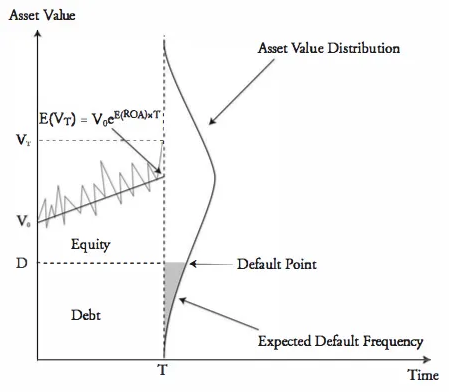
\includegraphics[width=0.8\linewidth]{img/KMV.png}
    \caption{企业债券的价值}\label{fig:bsm}
\end{figure}

模型的基本思路是:当企业期望市场价值$V$低于企业所需清偿的负债值$DP$时企业将发生违约。对公司价值和违约点的“距离”除以$V$,以对公司规模作了一个标准化,便于建立不同规模公司之间的对比;同时观察需要多少个$V$标准差的变化使得公司价值落在违约点以下,这就是到违约的距离。
\begin{equation}
    DD=\frac{V_A-DP}{V_A\sigma_A}\label{eq:dd}
\end{equation}
逐项来看公式(\ref{eq:dd}):
\begin{enumerate}
    \item 资产价值$V_A$和波动率$\sigma_A$的计算:将企业所有者权益视作欧式看涨期权,即\begin{equation*}
              E=\begin{cases}
                  V_A-D & V_A>D    \\
                  0     & V_A\le D
              \end{cases}
          \end{equation*}
          结合伊藤引理、企业股权价值本身服从几何布朗运动,可构造联立方程组得到\begin{eqnarray}
              E&=&V_AN(d_1)-e^{-rT}DN(d_2)\label{eq:ee}\\
              \sigma_E&=&\frac{V_A}{V_E} N(d_1)\sigma_A
          \end{eqnarray}其中$d_1=\frac{1}{\sigma_E\sqrt{T}}(\ln \frac{S}{L}+(\mu+\frac{1}{2}\sigma^2_E)T)$,$d_2=d_1-\sigma_E\sqrt{T}$
          所有者权益的价值和波动率都是公开的市场信息,从而可以计算得到$V_A$和$\sigma_A$
    \item $DP$的计算:违约点 D 需要考虑了流动性的影响,给长短债赋予不同的权重,将短期债务和长期债务考虑进去。KMV公司的计算方式为加总所有的短期负债(即到期日小于 1 年的)的面值加上 50\%长期债务的面值。
\end{enumerate}

如果资产价值服从对数正态分布,其连续增长率为$\mu$,公式(\ref{eq:dd})和(\ref{eq:ee})可以进一步化简为
\begin{equation}
    DD=\frac{\ln \frac{V_A}{DPT}+(\mu-\frac{1}{2}\sigma^2)T}{\sigma_A\sqrt{T}}\label{eq:f}
\end{equation}

得到违约距离$DD$后,KMV模型基于违约数据库,依据违约距离可以映射出公司实际的期望违约频率,例如历史上$DD=a$的公司有100个,其中有5个违约,那么$a$点的违约概率就为0.05。这种处理就对模型假设没有那么严格,也是与区别Merton模型最大的区别。 KMV 公司收集了包括3400上市公司和40000家非上市公司自1973年以来的资料,建立了庞大的数据库,得到从违约距离到预期违约率的映射关系,取得了良好的预测效果。

本文对KMV模型的改进在于对违约点的估计不再只是长期负债一半加上短期负债,以公司公司资产净利率ROA作为预期资产价值增长的速度$\mu$。

\subsection{KMV模型的价值}

KMV模型运用了现代期权定价理论,建立违约预测模型,综合考虑了经验和模型,降低了主观因素对信用评估的影响,是对传统信用风险度量方法的一次重要革命。股价中包含了投资者对于公司未来发展的预期,预期违约率中包含了投资者对信用状况未来发展趋势的判断,因此,该模型具有一定的前瞻性。KMV 模型的信用风险衡量指标预期违约率主要来自股票市场价格变化的有关数据,可以及时反映信用风险水平的变化。该模型主要依赖股票市场数据和财务报表中的负债数据进行计算,能够降低会计信息失真对模型结果的影响。

但KMV模型也存在一些缺陷,主要体现在以下三个方面中。
\begin{itemize}
    \item 首先,该模型假设公司的资产价值服从正态分布,但是事实上企业的资产价值经常会呈现出非正态的统计特征。
    \item 其次,模型的使用范围有一定的局限性。对上市公司而言,由于我国的股市有效程度较低,一方面许多上市公司的股价常常远超出公司的实际价值,另一方面企业资产价值特别是国有企业的资产价值并不能够完全反映到股票市值中,因而模型预测可能会被影响。而对非上市公司而言,往往要借助一些会计信息或其他能够反映借款企业特征值的指标来替代模型中一些重要变量,同时还要通过对比分析最终得出该企业的期望违约概率,一定程度上就有可能降低计算的准确性。
    \item 最后,模型不能区分不同类型的债务。不同类型债务之间由如偿还优先顺序、担保、契约等关系,KMV模型仅仅抽象出了短债和长债两个特征。
\end{itemize}

\section{实证与复现}

\subsection{数据预处理与描述性统计}

我国信用债市场曾经维持着“刚兑”神话,公开市场债券违约首现于2014年的11超日债违约,早于\citet{彭伟2012基于}写文章的日期。且截止至目前(\today),债券违约仍以非上市公司为主,如图\ref{fig:default}所示。因此\citet{彭伟2012基于}选择以公司是否被“ST”为违约标志。沪、深交易对财务状况和其他经营状况异常的上市公司的股票交易进行特别处理(Special Treatment),以表明比一般正常的上市公司具有较高的投资风险。实际情况中,虽然公司信贷违约与被 ST、*ST 不完全等同,但他们之间有较强的相关性,如超日债即为ST超日2011年发行的债券。
\begin{figure}[H]
    \centering
    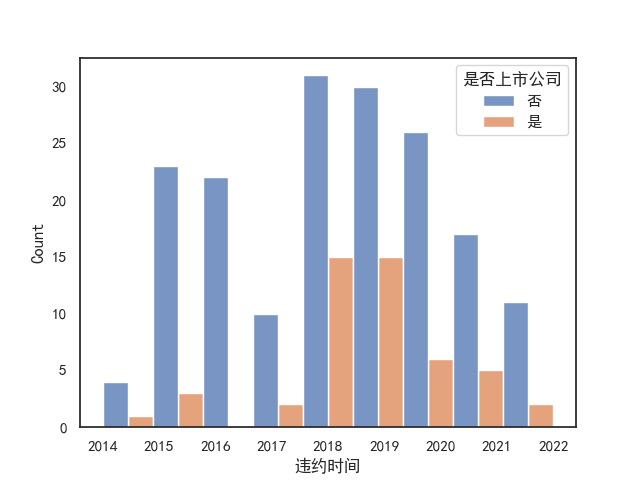
\includegraphics[width=\linewidth]{img/发行人首次债券违约.png}
    \caption{迄今为止发行人首次债券违约时间分布}\label{fig:default}
\end{figure}

采用是否ST衡量公司违约有一定的问题,这是由于当时数据的局限性造成的。但实施ST的原因与公司信贷违约尚有差距,如连续亏损、含非标意见等。尽管这些情形可能是公司走向违约等标志,但ST股票的判定和撤销取决于交易所的判断,交易所对风险的理解会影响到一家公司是否被ST。后验地看不少公司在公开市场违约时仍尚未被ST,如华夏幸福、泰禾、蓝光等企业,更遑论更一般的信贷市场违约(公开债务违约前往往是非公开债务如信托、银行贷款违约)时。时至今日我国信贷违约数据库尚在建设中,公开市场虽然打破了刚兑但数据量难以支撑大模型,这也是KMV模型应用的挑战之一。
\begin{table}[H]
    \centering
    \begin{tabular}{lcc}
        \toprule
        符号   & 经营连续亏损 & 预警           \\
        \midrule
        *ST  & 三年     & 退市预警         \\
        ST   & 二年     & 特别处理         \\
        S*ST & 三年     & 退市预警+还没有完成股改 \\
        SST  & 二年     & 特别处理+还没有完成股改 \\
        \bottomrule
    \end{tabular}
    \caption{沪深交易所对ST/*ST的规定}
\end{table}

清理数据后,共有89家满足\citet{彭伟2012基于}中小企业的定义(原文中有111家):
\begin{enumerate}
    \item 2008 年 1 月 1 日之前在沪深证券交易所上市
    \item 流通股 ≤ 5 000 万股,且 2007 年 12 月31日前的主营收入或资产总额≤5 亿元。
    \item 删除那些停牌时间较长的公司,
    \item 没有 B 股、H 股股票
\end{enumerate}

再进一步剔除掉股权波动率为0的样本点,数据描述性统计如图\ref{fig:des1}和图\ref{fig:des2}所示,其中波动率采用了GARCH(1,1)模型计算得出,对于股权的价值,作者参考\citet{张绍敏2007基于违约距离的财务预警模型},考虑我国的国情,将非流通股也纳入考虑,并对非流通股做了一定的折价,即股权价值= 流通股市值 +(0.99576+0.60973$\times$每股净资产)$\times$非流通股数。
\begin{figure}[H]
    \centering
    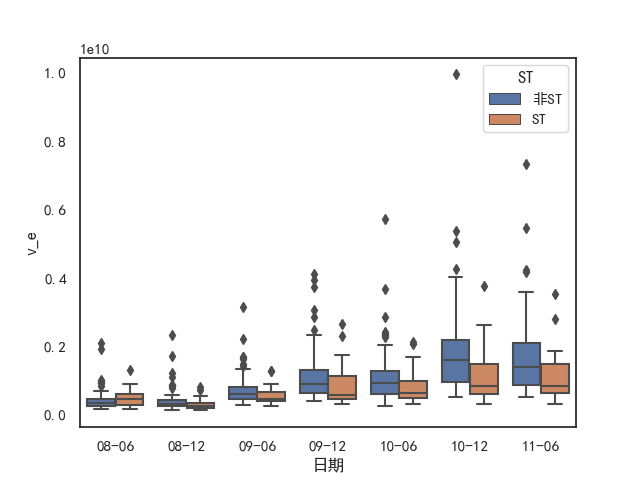
\includegraphics[width=0.8\textwidth]{img/v_e.png}
    \caption{股权价值}\label{fig:des1}
\end{figure}
\begin{figure}[H]
    \centering
    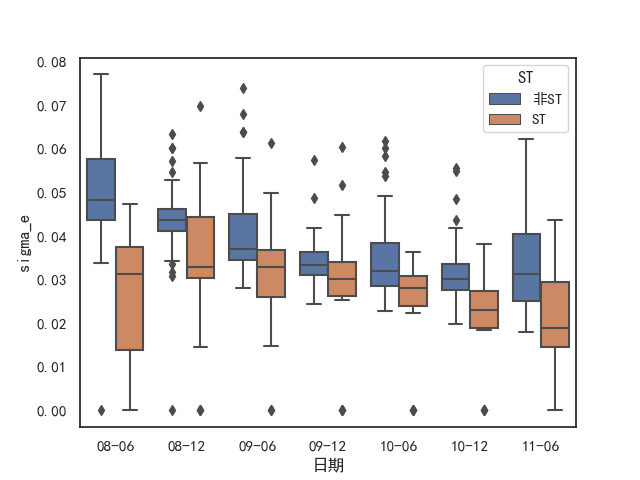
\includegraphics[width=0.8\textwidth]{img/sigma_e.png}
    \caption{股权价值波动率}\label{fig:des2}
\end{figure}

对于债权的价值,作者对所有08-11年的所有被实施ST的股票的总资产、短期负债和长期负债的价值进行了多元线性回归。复现结果如表\ref{tab:1}所示,与作者的$DPT = 1.11\times SD+0.65\times LD$接近,均大于KMV公司的原始数据,说明我国中小上市企业信贷风险相对国外更高,也可以说交易所判定是否ST较为严格。
\begin{table}[H]
    \small\begin{center}
\begin{tabular}{lclc}
\toprule
\textbf{Dep. Variable:}    &       总资产        & \textbf{  R-squared (uncentered):}      &     0.968   \\
\textbf{Model:}            &       OLS        & \textbf{  Adj. R-squared (uncentered):} &     0.968   \\
\textbf{Method:}           &  Least Squares   & \textbf{  F-statistic:       }          &     4304.   \\
\textbf{Date:}             & Wed, 23 Nov 2022 & \textbf{  Prob (F-statistic):}          & 5.84e-211   \\
\textbf{Time:}             &     11:05:32     & \textbf{  Log-Likelihood:    }          &   -6294.1   \\
\textbf{No. Observations:} &         282      & \textbf{  AIC:               }          & 1.259e+04   \\
\textbf{Df Residuals:}     &         280      & \textbf{  BIC:               }          & 1.260e+04   \\
\textbf{Df Model:}         &           2      & \textbf{                     }          &             \\
\textbf{Covariance Type:}  &    nonrobust     & \textbf{                     }          &             \\
\bottomrule
\end{tabular}
\begin{tabular}{lcccccc}
               & \textbf{coef} & \textbf{std err} & \textbf{t} & \textbf{P$> |$t$|$} & \textbf{[0.025} & \textbf{0.975]}  \\
\midrule
\textbf{流动负债}  &       1.3733  &        0.033     &    41.761  &         0.000        &        1.309    &        1.438     \\
\textbf{非流动负债} &       0.8951  &        0.053     &    16.821  &         0.000        &        0.790    &        1.000     \\
\bottomrule
\end{tabular}
\begin{tabular}{lclc}
\textbf{Omnibus:}       & 174.038 & \textbf{  Durbin-Watson:     } &    1.984  \\
\textbf{Prob(Omnibus):} &   0.000 & \textbf{  Jarque-Bera (JB):  } & 3432.492  \\
\textbf{Skew:}          &   2.077 & \textbf{  Prob(JB):          } &     0.00  \\
\textbf{Kurtosis:}      &  19.579 & \textbf{  Cond. No.          } &     3.41  \\
\bottomrule
\end{tabular}
%\caption{OLS Regression Results}
\end{center}

Notes: \newline
 [1] R² is computed without centering (uncentered) since the model does not contain a constant. \newline
 [2] Standard Errors assume that the covariance matrix of the errors is correctly specified.
    \caption{债权价值复现}\label{tab:1}
\end{table}

最后,作者将负债的平均期限假定为一年,企业预期资产价值增长的速度为公司资产净利率。资产价值增长速度理论依据是\citet{夏红芳2007基于},其对比了采用ROA和无风险利率的算法,发现对于农业公司而言,采用ROA的方式更适合我国国情,且误差较小。
\begin{figure}[H]
    \centering
    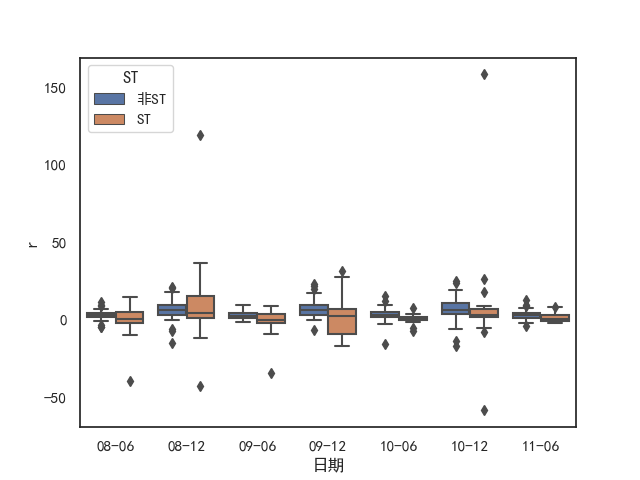
\includegraphics[width=0.8\textwidth]{img/r.png}
    \caption{公司资产净利率}
\end{figure}
\subsection{中小上市企业的违约距离}

数据代入公式(\ref{eq:f})计算出整体不同年份的的违约距离如图\ref{fig:dd}所示,而对不同的年份的ST与非ST股票的违约距离均值则如图\ref{fig:st},ST和非ST股票在违约距离均值上有差异。检查违约距离较低的如非ST股票在后来也逐渐沦为ST股票,如ST新智、ST冠福、ST天宏等。由于彼时中国市场尚存在刚兑神话,即便放宽违约为被ST仍数量有限,难以通过违约距离$DD$得到相应的违约概率,因此作者停在这一步,用违约距离这一指标来衡量公司的信贷风险,并在之后的工作\cite{彭伟2012我国上市中小企业信贷风险研究}中进一步揭示有效性。
\begin{figure}[H]
    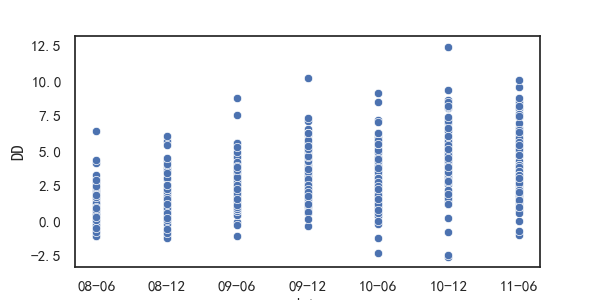
\includegraphics[width=\linewidth]{img/dd.png}
    \caption{整体公司的违约距离}\label{fig:dd}
\end{figure}
\begin{figure}[H]
    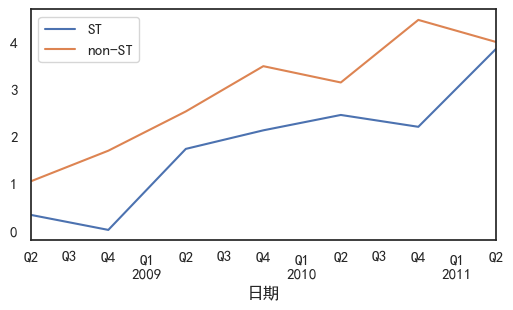
\includegraphics[width=\linewidth]{img/st-vs-non-st.png}
    \caption{ST与非ST公司的违约距离均值}\label{fig:st}
\end{figure}

而对KMV模型是否有效,作者采用了两个独立样本的K-S检验和Mann-Whitney检验,结果如图\ref{fig:origin},作者的K-S检验前 6 个半年及Mann-Whitney检验7个半年的P值均小于0.05,只有K-S 检验的 2011年上半年双尾检验概率 P 值为0.067。K-S检验的显著性差异证明ST与非ST公司的违约距离不是同一个分布,MW检验显著性则验证了样本的均值并非相等。
\begin{figure}[H]
    \begin{minipage}{0.48\linewidth}
        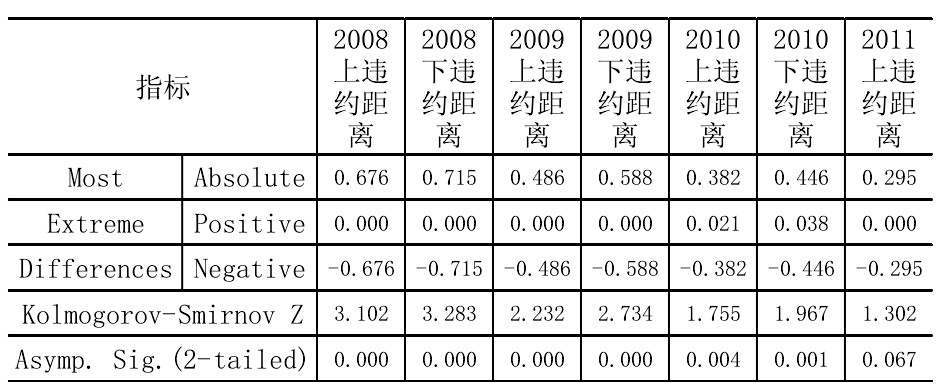
\includegraphics[width=\linewidth]{img/ks.jpeg}
    \end{minipage}
    \begin{minipage}{0.48\linewidth}
        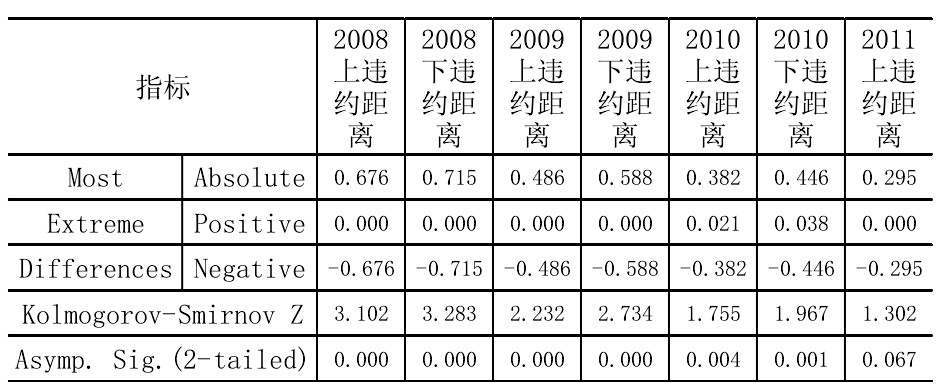
\includegraphics[width=\linewidth]{img/mw.jpeg}
    \end{minipage}
    \caption{原文中的KS(左)和MW(右)检验的结果}\label{fig:origin}
\end{figure}

但复现结果分别如表\ref{tab:KS}和表\ref{tab:MW}所示,显著性不强,可能由于样本数差异或数据处理方法差异,仅在部分年份显著,大部分时间表现显著性较弱。
\begin{table}[H]
    \centering
    \begin{tabular}{lrrrrrrr}
\toprule
{} &  2008-06-30 &  2008-12-31 &  2009-06-30 &  2009-12-31 &  2010-06-30 &  2010-12-31 &  2011-06-30 \\
\midrule
statistic &    0.277778 &    0.222222 &    0.222222 &    0.194444 &    0.291667 &    0.291667 &    0.208333 \\
pvalue    &    0.236850 &    0.384915 &    0.384915 &    0.472853 &    0.206561 &    0.206561 &    0.427943 \\
\bottomrule
\end{tabular}

    \caption{两个独立样本的K-S检验}\label{tab:KS}
\end{table}
\begin{table}[H]
    \centering
    \begin{tabular}{lrrrr}
    \toprule
    {}        & 2008-06-30 & 2008-12-31 & 2009-06-30 & 2009-12-31 \\
    statistic & 158.000000 & 47.000000  & 135.000000 & 78.000000  \\
    pvalue    & 0.230442   & 0.005167   & 0.284836   & 0.028662   \\
    \midrule
    {}        & 2010-06-30 & 2010-12-31 & 2011-06-30 &            \\
    statistic & 182.000000 & 131.000000 & 217.000000 &            \\
    pvalue    & 0.443427   & 0.091772   & 0.892414   &            \\
    \bottomrule
\end{tabular}

    \caption{Mann-Whitney检验}\label{tab:MW}
\end{table}

\subsection{违约风险的影响因素}
作者对违约风险的归纳主要是从公式(\ref{eq:dd})出发的,将未来的资产价值与资产的隐含波动率还原为总资产和股价波动的影响,研究二者对违约的影响。复现结果如表\ref{tab:asset}和\ref{tab:vol}所示,后者与论文结果类似。
\begin{table}[H]
    \centering
    \begin{tabular}{lrrrr}
    \toprule
    {}       & 2008-06-30 & 2008-12-31 & 2009-06-30 & 2009-12-31 \\
    pearsonr & -0.265334  & -0.221167  & -0.410335  & -0.230768  \\
    pvalue   & 0.016667   & 0.047233   & 0.000142   & 0.038201   \\
    \midrule
    {}       & 2010-06-30 & 2010-12-31 & 2011-06-30 &            \\
    pearsonr & -0.354095  & -0.444828  & -0.464128  &            \\
    pvalue   & 0.001182   & 0.000032   & 0.000013   &            \\
    \bottomrule
\end{tabular}

    \caption{违约距离与总资产的相关系数}\label{tab:asset}
\end{table}
\begin{table}[H]
    \centering
    \begin{tabular}{lrrrr}
\toprule
{} &  2008-06-30 &  2008-12-31 &  2009-06-30 &  2009-12-31  \\
pearsonr &   -0.023419 &   -0.312969 &   -0.254424 &   -0.184716\\
pvalue   &    0.835603 &    0.004444 &    0.021901 &    0.098770\\
\midrule
{} &  2010-06-30 &  2010-12-31 &  2011-06-30 &\\
pearsonr &  -0.249410 &   -0.121688 &   -0.327771& \\
pvalue   &   0.024741 &    0.279166 &    0.002817& \\
\bottomrule
\end{tabular}

    \caption{违约距离与股价波动率的相关系数}\label{tab:vol}
\end{table}

公司规模理应是影响公司信用风险的重要因素。资产规模较大的公司一般而言具有更强的变现能力,因而其相应的违约距离也就更大。并且在实际的信贷市场中,大公司向银行争取贷款相对于中小企业而言显得更为容易,这也正是中小企业在信贷市场上“融资难、融资贵”,导致其信贷风险偏高的原因。但是复现结果显现其资产规模越大,其违约距离却相对更低。可能的原因为中小企业资产规模相对都较小,其中的资产规模相对大的企业资产的波动率也更大。

股权市场上的波动率对KMV模型也有较大的影响,波动率越高违约距离越小。这可能是由于股权价值的高波动导致资产价值到预期违约距离的标准差倍数越小。

但是,违约风险并非只与KMV模型相关。2008-2011是金融危机冲击后的时代,正如图\ref{fig:dd}中所展示的,2008年时中小企业整体的违约距离更低,宏观层面对整体信贷风险会有比较大的影响。或许由于写作时代的原因,作者并未涉及到宏观环境对公司信贷风险的影响。学者诸如\citet{bai2019common} 和\citet{bali2021macroeconomic}分别从宏观经济下行和宏观经济不确定性出发,研究宏观环境对于公司债利差的影响。\citet{王博2019货币政策不确定性}指出货币政策不确定性的增加会带来违约风险的上升。\citet{梅冬州2021财政扩张} 和\citet{2020Fiscal} 则认为财政扩张导致挤出效应,从而民企面临融资困境,进而违约率上升,利差走阔。

最后,流动性和系统性风险可能会影响违约\cite{brogaard2017stock},更高的流动性可以通过提高价格效率来降低违约风险,或者通过放松投资者的退出能力来改善公司治理。\citet{苟文均2016债务杠杆与系统性风险传染机制}基于 CCA 模型,提出杠杆率应从较高居民转移至政府等低杠杆部门,以降低违约风险。\citet{2020Do}基于 VaR 模型,认为几乎所有的系统性风险指标对对违约率都有预测能力。

\subsection{违约距离对信贷风险的预测效果}
在论证了KMV模型中的违约距离与信贷风险相关后,作者进一步想验证违约距离对信贷风险的预测能力。于是作者选择数据中2010-2011年间被ST的样本,研究其在被ST前的5个半年内违约距离DD值的变化规律。但数据选择有误,实际2010下半年和2011上半年仅有两个公司满足条件:ST天润(2010-10-20)和 *ST大地(2011-05-04)
\begin{figure}[H]
    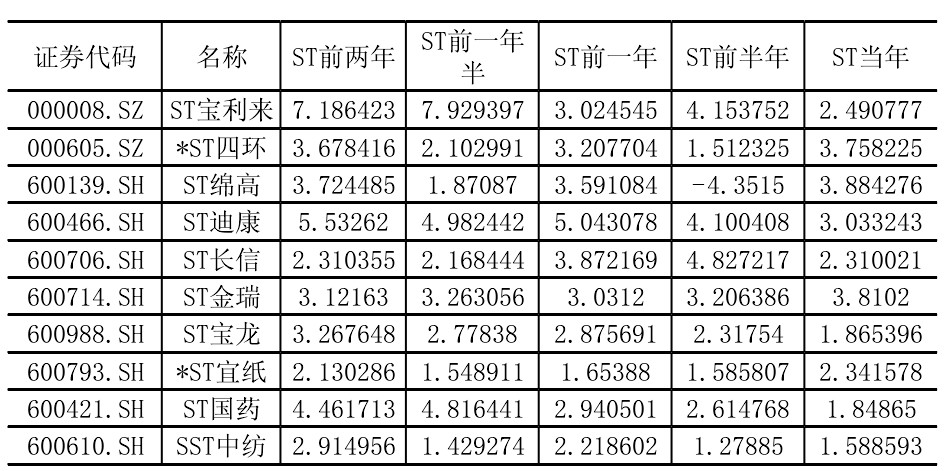
\includegraphics[width=\linewidth]{img/dd_origin.jpeg}
    \caption{原论文称这些公司为2010-2011年间被ST,但事实上均2008年便被ST}
\end{figure}
\begin{table}[H]
    \centering
    \begin{tabular}{lcc}
        \toprule
               & ST天润     & *ST云投    \\
        \midrule
        ST前两年  & 0.238944 & 2.106469 \\
        ST前一年半 & 1.547428 & 4.392480 \\
        ST前一年  & 1.779768 & 3.959906 \\
        ST前半年  & 2.275831 & 2.631978 \\
        ST当年   & 1.222579 & 1.927210 \\
        \bottomrule
    \end{tabular}
    \caption{事实上的满足条件样本的违约距离}
\end{table}

复现结果在ST前一年半内表现较好,违约距离整体呈现走低的趋势。但是考虑到两年全量,表现差强人意。可能的解释是考虑两年时,金融危机的影响较大,因而导致整体的违约距离较低。
\begin{figure}[H]
    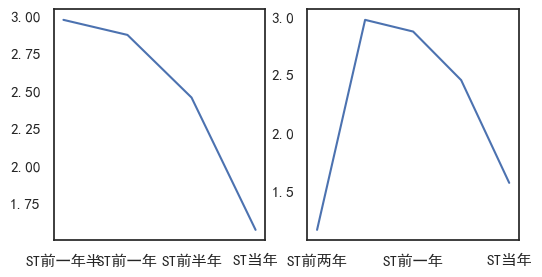
\includegraphics[width=\linewidth]{img/st.png}
    \caption{一年半内持续走低,两年全量不明显}
\end{figure}

作者还做了频率统计(图\ref{fig:origin23}),发现违约距离越小,ST的频率就越高,与KMV模型一致,因而作者提出可以设置信贷风险预警线:$DD=2$为二级预警线,而$DD=1$为一级预警线,低于二级预警线有47\%的概率被ST,而低于一级预警线有81\%的概率被ST。2011年上半年有32.67\%的中小企业违约距离低于二级警戒线。复现结果(图\ref{fig:23})显示并非如此,后验视角看也没有$47\%\times 67\% = 31.49\%$的样本内企业被ST。
\begin{figure}[H]
    \begin{minipage}{0.48\linewidth}
        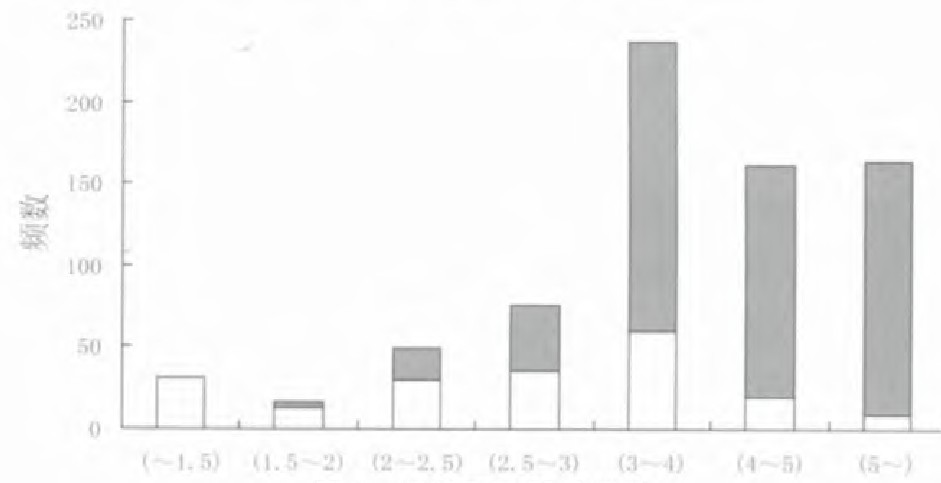
\includegraphics[width=\linewidth]{img/fig2.jpeg}
    \end{minipage}
    \begin{minipage}{0.48\linewidth}
        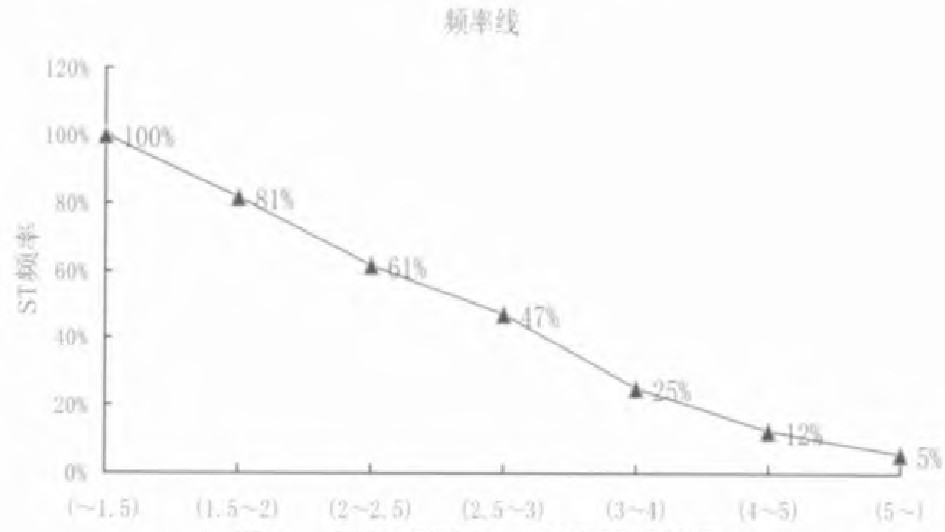
\includegraphics[width=\linewidth]{img/fig3.jpeg}
    \end{minipage}
    \caption{作者ST频数(左)与频率(右)分布图,横轴为$DD$}\label{fig:origin23}
\end{figure}
\begin{figure}[H]
    \begin{minipage}{0.48\linewidth}
        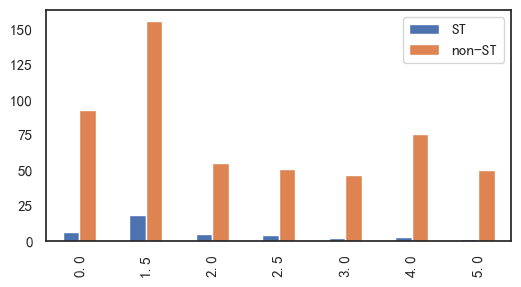
\includegraphics[width=\linewidth]{img/fig2_.png}
    \end{minipage}
    \begin{minipage}{0.48\linewidth}
        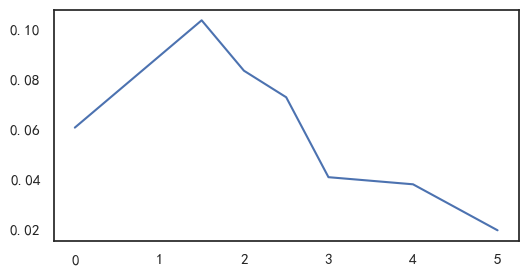
\includegraphics[width=\linewidth]{img/fig3_.png}
    \end{minipage}
    \caption{复现ST频数(左)与频率(右)分布图,横轴为$DD$}\label{fig:23}
\end{figure}

预测的准确性方面,作者建立了一个临界值模型。具体地说,作者设定违约距离临界值为$0.5\times \bar{DD}_t+0.5\times 3$,低于该临界值则预测公司违约。当然考虑到违约距离的误差,作者在判断I类错误时将阈值上调0.3,而判断II类错误时阈值下调0.3,其结果如图\ref{fig:error}所示。复现结果如表\ref{fig:myerror}所示。
\begin{figure}[H]
    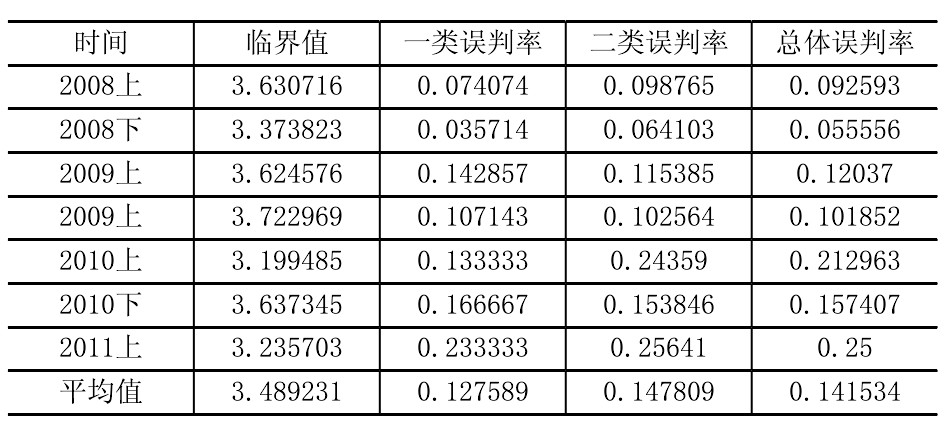
\includegraphics[width=\linewidth]{img/tab1.jpeg}
    \caption{作者的I/II类错误误判率}\label{fig:error}
\end{figure}
\begin{table}[H]
    \centering
    \begin{tabular}{lrr}
\toprule
{} &     $\alpha$ &      $\beta$ \\
\midrule
2008-06-30 &  0.000000 &  0.800000 \\
2008-12-31 &  0.000000 &  0.723684 \\
2009-06-30 &  0.200000 &  0.631579 \\
2009-12-31 &  0.000000 &  0.539474 \\
2010-06-30 &  0.333333 &  0.560000 \\
2010-12-31 &  0.333333 &  0.386667 \\
2011-06-30 &  0.666667 &  0.506667 \\
\bottomrule
\end{tabular}

    \caption{复现的I/II类错误误判率}\label{fig:myerror}
\end{table}

\subsection{反思与尝试}

回顾这篇文章,作者参考\citet{夏红芳2007基于},采用公司资产净利率作为企业价值的预期增长率。但公司资产净利率本身是一个滞后性指标,只有企业在公布财报后才会有所显现,通常会滞后选取的时间点2-3个月,例如3月左右才会公布上年的公司资产净利率。已有的研究更多是以无风险利率作为企业价值的预期增长率,我认为无风险利率更为合理,更能满足BSM公式的无套利假设。因而采用隔夜拆借利率,将工程文件中的 dataloader.py中的 Dataloader.mappings 进行修改后即成为调用无风险利率,具体如下所示。复现结果与使用公司资产净利率类似,但相对更为及时。
\begin{figure}[H]
    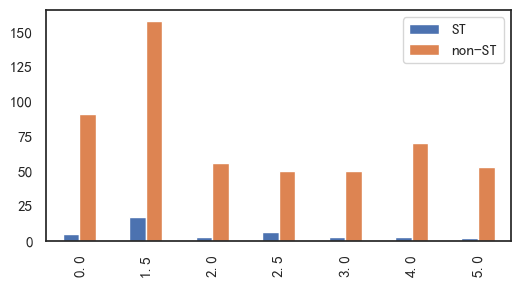
\includegraphics[width=\linewidth]{fig/output.png}
    \caption{采用无风险利率结果与采用ROA基本一致}
\end{figure}
\begin{minted}{python}
class Dataloader:
    mappings = {
        "v_a": "资产价值",
        "v_e": "股权价值",
        "sigma_a": "资产价值波动率",
        "sigma_e": "股权价值波动率",
        "d": "债务价值",
        "r": "隔夜拆借利率",
        "assets": "资产规模",
    }
    ...
\end{minted}

\section{心得与感悟}
经验与模型哪个重要正如剑宗与气宗之争,基本面重要还是市场面重要也正如哲学中唯物与唯心的探讨。不过无论怎样,模型都是来源于过去的经验总结,从经验中来最终也会化归到经验中去。经验与模型是相辅相成的关系,所以我们需要结合经验与模型来对中国特色的信贷市场进行估值和分析,同时强调基本面与市场面结合交叉检验的风险分析框架。
\begin{figure}[H]
    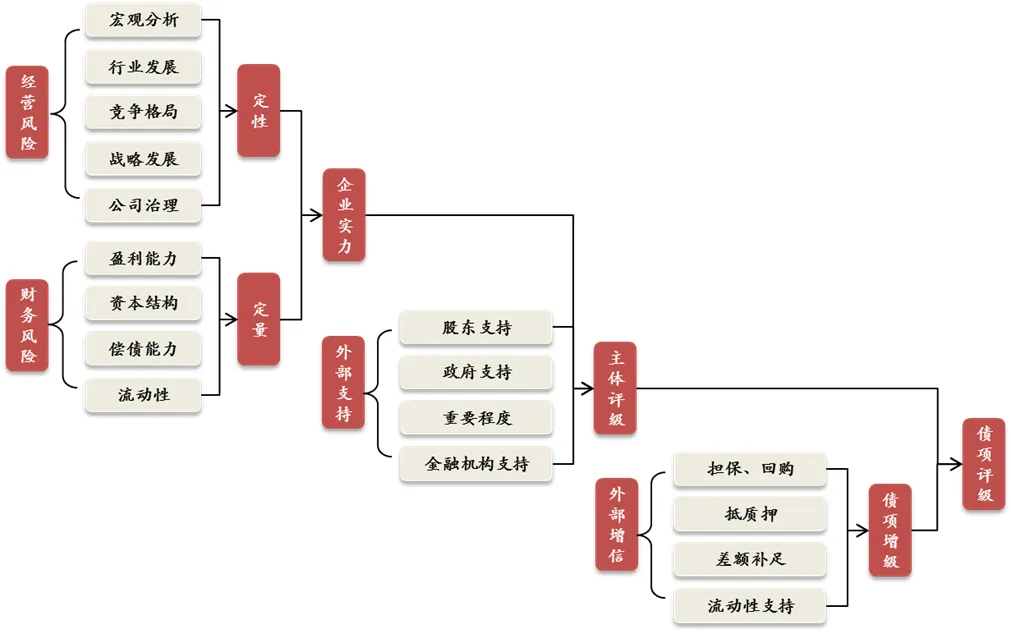
\includegraphics[width=\linewidth]{fig/信用研究框架.png}
    \caption{典型的信用研究框架}
\end{figure}

就本文而言,可能的改进方向有以下几点:
\begin{enumerate}
    \item 对信贷风险进一步落实。尽管信贷数据主要位于各国有大行手中,公开市场债券违约数据已经相对充足。可以延展到更多样本的时间序列上来观察股价波动、事件冲击(评级调整、信用事件)、财报公布等对公司违约距离的影响,例如20年11月的永煤违约、22年11月的理财赎回潮均债券市场大幅波动,不少企业不得不取消发行债券,可能使得部分主体违约距离承压。
    \item 违约距离与个券收益率走势的交叉检验。可以对发行人所发行的所有债券根据其期限、余额,估值等指标构建一个加权债券指数作为其债券市场走势,与股价、违约距离三者进行交叉检验,来判断同一公司不同资产价格变动的共同趋势与差异。
    \item 增添行业补偿系数进行行业调整。KMV模型归根结底是根据资产价格是否击穿权益安全垫来判断违约风险。本文采用流动负债与非流动负债的加权比例来作为违约点。而众所周知的是,不同行业负债结构差别很大,不能一概而论。运用广泛的行业打分体系也是分行业来进行财务横向比较,跨行业比较较易失真,所以当样本公司进一步增多后,应当增添行业对KMV模型的修正。
\end{enumerate}
限于时代背景,作者研究信用风险的标准是被ST的股票。随着公开市场债券打破刚兑、资管理财产品净值化,以及宏观环境与政策冲击,后疫情时代波动率显著上升,中资高收益债走入了至暗时刻,大量的企业债券违约,大量的贷款成为坏账,甚至对中国宏观经济造成了一定的影响。我们拥有了更多的违约数据,所谓“前事不忘。后事之师”,当前压垮这些企业的那些最重的那根稻草,对避免未来相似的场景重新发生,也有一定的借鉴意义。KMV模型为我们提供了一些思路,让我们思考资产的波动对企业信贷风险的影响。
\begin{figure}[H]
    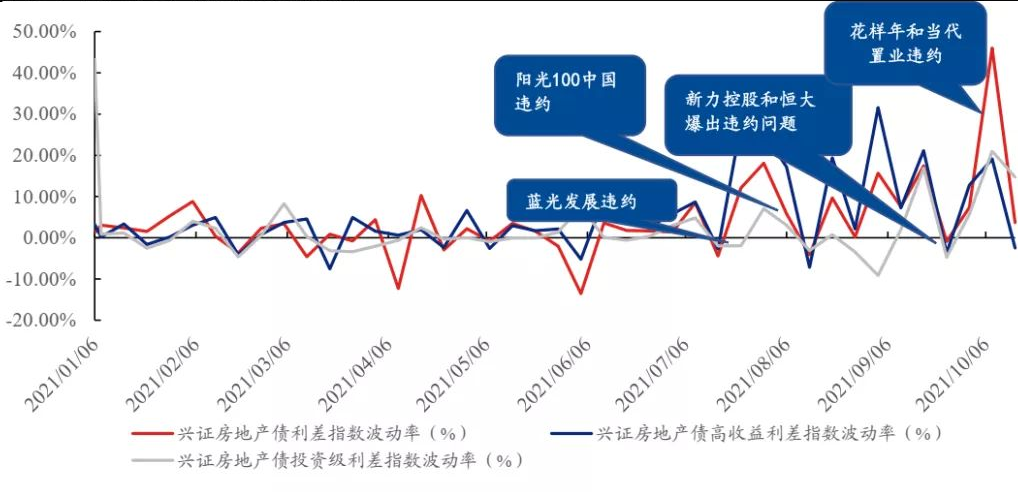
\includegraphics[width=0.8\linewidth]{fig/波动率.jpeg}
    \caption{大波动的时代}
\end{figure}

最后,KMV 模型反应了信用评价方法从定性的经验判断向定量的指标衡量发展,从单一的历史财务数据分析到考虑多种信用影响因素。KMV模型通过引入股票市场价格实时行情来判断投资者对该企业未来发展的综合预期,但大部分发债企业并非上升公司,同时在新兴市场,股票价格的波动剧烈,并不完全反映企业的真实情况,需要认识到单一评价方法的不足,在信用评价过程中,要结合外部经济环境、行业发展趋势、企业的财务表现进行综合评价。

\nocite{*}
\appendix
\printbibliography%[heading=bibliography,title=参考文献]
\end{document}
